
\subsection{Método de ventanas}

Se desea implementar el ecualizador mediante un filtro que no agregue distorsión de fase. Para ello se utilizan los filtros \emph{FIR FLG}. En esta sección se diseña y caracteriza un filtro mediante el método de ventanas.

% \lstinputlisting[firstline=30, lastline=76]{tp.m}

	\subsubsection{Ítem a: amplitud del ecualizador}

% Definir A_{EQ}(w) con sus correspondientes bandas, amplitudes, tolerancias (ripple) adecuadas para cumplir los requerimientos, frecuencias de corte, paso y supresión.

%La frecuencia de muestreo es de $f_s = \SI{44.1}{\kilo\Hz}$. 
	Primero se realiza la transformada rápida de Fourier o \textit{fft} de 1024 puntos de la señal que entrega el sistema electroacústico. Esta señal es la que se tiene como dato en el archivo \textit{SEA.mat}.\\

Para obtener las bandas de interés, se calculan los extremos locales de esta curva, teniendo en cuenta que se puede acotar el rango de frecuencias de interés de la señal desde los $\SI{20}{\Hz}$ hasta los $\SI{16}{\kilo\Hz}$\footnote{El rango audible de frecuencias para el humano adulto es $\SI{20}{\Hz}$ - $\SI{20}{\kilo\Hz}$. Para los fines de este trabajo práctico, se ha decidido acotar un poco más las frecuencias agudas al valor mencionado.}, ya que se trata de una señal de audio.\\

	\graficarEPS{0.6}{graf_P11a_sistema_EA}{Módulo de la respuesta en frecuencia del sistema electroacústico original.}{fig:P11a_sistema_EA}
	
	Como primera aproximación, se obtienen los extremos utilizando la función \textit{findpeaks}, que devuelve tanto la ubicación de cada máximo como el valor del mismo. Para hallar los mínimos, se aplica la misma función pero al módulo de la respuesta inversa del sistema. Luego, los límites de las bandas para el filtro son los valores promedio entre cada máximo y mínimo consecutivo. En la Figura \ref{fig:P11a_sistema_EA} se muestra el resultado de dicho proceso.\\

% La curva azul representa el módulo de la respuesta en frecuencia del sistema electroacústico; en verde se marcan los límites de las frecuencias de interés mencionadas, escaladas según el valor de la frecuencia de muestreo; los puntos rojos son los extremos locales obtenidos; las bandas de interés están delimitadas por las líneas punteadas amarillas.\\

%	En la Figura \ref{fig:P11a_sistema_EQ} se muestra la respuesta del filtro multibanda y la del sistema original:
%
%	\begin{figure} [H]
%		\centering
%		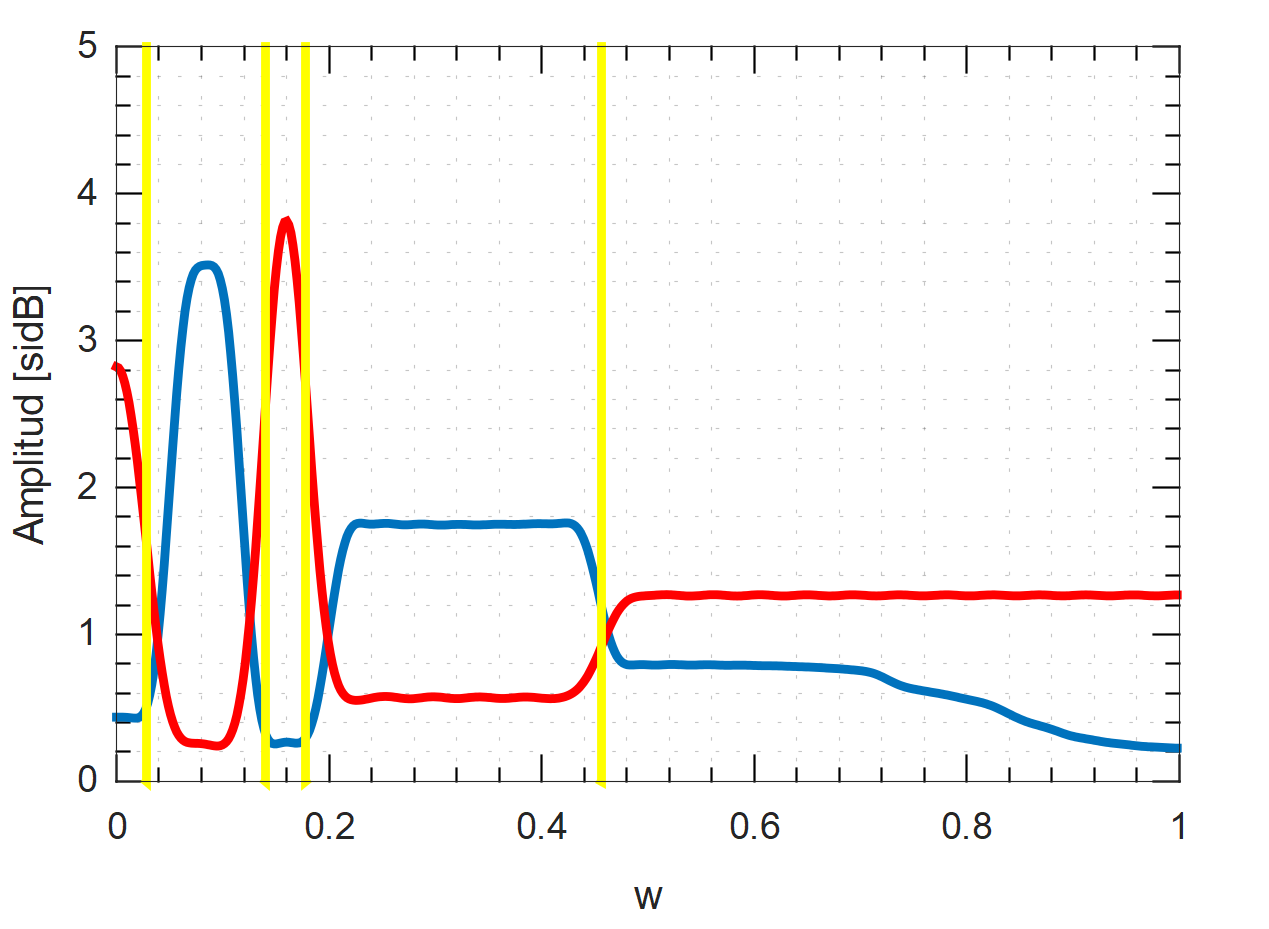
\includegraphics[width=0.9\textwidth]{P11a_sistema_EQ.png}
%		\caption{\label{fig:P11a_sistema_EQ}Módulo de la respuesta en frecuencia del filtro ecualizador y del sistema electroacústico original.}
%	\end{figure}
%
%La curva azul representa el módulo de la respuesta en frecuencia del sistema electroacústico; la curva roja representa la del filtro multibanda diseñado; las bandas de interés están delimitadas por las líneas amarillas.\\
%
%Se obtienen los siguientes valores para los parámetros de cada banda:
	
	Según hipótesis, la tolerancia es de \SI{2}{\dB} que equivale a $\delta_0 = 0.01$ de magnitud. Sin embargo, para la utilización de ventanas se debe hacer un escalamiento de las tolerancias correspondientes a cada banda. Para normalizar las tolerancias $\delta$ del sistema electroacústico, se realiza el cociente $\delta_i = \delta_0 / a_i$ donde $a_i$ es la ganancia de la i-ésima banda.\\

	En la Tabla \ref{tab:specs} se exponen las caracterísitcas de la función amplitud $A_{EQ}(w)$ del filtro a implementar. Por inspección se obtiene que $\max \{\delta_i\} = \delta_3 \approx 0.04$. Este valor implica que no hay restricción de qué ventana utilizar, dado que la que tiene el $\delta$ más pequeño es la \emph{rectwin} con $\delta_{rectwin} = 0.09$ y es mayor que $\delta_3$.

	Por último se decidió no definir las bandas de paso y supresión de cada caso. En el caso que fuese necesario obtener estos valores, se obtendrán a partir del valor de $w_c$ y la suma (o resta) de un $\Delta w = \num{0.025}\cdot\pi$.

	\begin{table}[h!]
		\centering
		\begin{tabular}{*{6}{c}}
			\toprule
			Parámetro	&	Banda 1 & Banda 2 & Banda 3 & Banda 4 & Banda 5\\
			\midrule
			Frecuencias límites ($\frac{w_c}{\pi}$)	& $0$ - $0.050$	& $0.050$ - $0.120$	& $0.120$ - $0.203$	& $0.203$ - $0.456$	& $0.456$ - $0.726$\\
			Ganancia		& $2.327$	& $0.284$	& $3.933$	& $0.569$	& $1.267$\\
			Tolerancia ($\delta_i$)	& $0.023$	& $0.003$	& $0.039$	& $0.006$	& $0.013$\\
			\bottomrule
		\end{tabular}
		\caption{Especificaciones para el filtro a implementar.}
		\label{tab:specs}
	\end{table}


	\subsubsection{Ítem b: filtro multibanda}

	Previo a la construcción del filtro ecualizador, se diseña la función \texttt{multibanda(a,w,M,win)} que se encarga de generar el filtro deseado a partir de suma y/o restas de filtros pasa-bajos. Para corroborar el correcto funcionamiento de dicha función, se propone generar un filtro cuya respuesta en frecuencia coincida con la respuesta del sistema. De este modo se puede también verificar que los datos especificados en la Tabla \ref{tab:specs} sean correctos (utilizando como alturas la inversa de las ganancias expuestas en dicha Tabla).\\

	Como la longitud del lóbulo principal más pequeño de la respuesta del sistema electroacústico (segunda banda) se supuso como $\Delta w = 0.1\pi$, para una ventana rectangular se obtiene que $M_{rectwin}=41$. En la Figura \ref{fig:P11b_seguidor_rectwin} se presenta el filtro que sigue la respuesta del sistema utilizando la ventana rectangular. 
	
	Dado que el \emph{ripple} generado por la ventana es mayor a la tolerancia aceptable, se opta por seguir a la señal por medio de una ventana de \emph{Hamming}. Se puede ver en la Figura \ref{fig:P11b_seguidor_hamming} que al aumentar el orden, el filtro consigue replicar el comportamiento de la respuesta del sistema. Las diferencias pueden deberse al efecto de los lóbulos secundarios que disminuyen los valores pico de la segunda y tercer banda. Con un ajuste de las amplitudes podría conseguirse una curva más cercana.\\
	
	\HgraficarEPS{0.6}{graf_P11b_seguidor_rectwin}{Seguimiento de la respuesta del sistema EA por medio de \texttt{multibanda()} utilizando ventana rectangular.}{fig:P11b_seguidor_rectwin}
	
	\HgraficarEPS{0.6}{graf_P11b_seguidor_hamming}{Seguimiento de la respuesta del sistema EA por medio de \texttt{multibanda()} utilizando ventana de \emph{Hamming}.}{fig:P11b_seguidor_hamming}

	\pagebreak
	A partir del análisis expuesto en el párrafo anterior, y el ajuste de los parámetros, se obtiene el filtro ecualizador $H_{EQ}(w)$ utilizando $M=90$ y ventaneo de \emph{Hamming}. Se decidió por el filtro de tipo I (orden par; simétrico), para que no atenúe las frecuencias en $0$ ni en $\pi$. 
	De todas formas, si se hubiese implementado un filtro tipo II, al no poder escuchar tan bajas frecuencias (por el cero en 0), no sería un inconveniente.
	En la Figura \ref{fig:P11c_rta_frecuencia_eq} se ilustra el filtro ecualizador en conjunto con la respuesta del sistema. Al final de esta sección se provee una fracción del código utilizado para generar los gráficos expuestos con los respectivos parámetros.	

	\graficarEPS{0.6}{graf_P11c_rta_frecuencia_eq}{Módulo de la respuesta en frecuencia del filtro ecualizador.}{fig:P11c_rta_frecuencia_eq}

	\begin{lstlisting}
aux=[H(LOC2(1)) H(LOC(1)) H(LOC2(2)) H(LOC(2)) H(LOC2(end))];
% Copia de HSEA
%%%% RECTWIN %%%%
%	M = 41;
%	wc = [0.050 0.120 0.193 0.456];
%	a = aux;
%	tipo_ventana = @rectwin;
%
%%%% HAMMING %%%%
%	M = 90;
%	wc = [0.050 0.120 0.193 0.456];
%	a = aux;
%	tipo_ventana = @hamming;

%% Filtro ecualizador
	M = 90;
	wc = [0.028 0.140 0.178 0.456];
	a = [3.00 0.260 04.83 0.569 1.266];
	tipo_ventana = @hamming;

[heq, M] = multibanda(a,wc,M,tipo_ventana);
	\end{lstlisting}

	\subsubsection{Ítem c: respuesta en frecuencia y retardo de fase}
	
	Una vez implementado el filtro multibanda deseado, ilustrado en la Figura \ref{fig:P11c_rta_frecuencia_eq}, se calcula el producto de la respuesta del sistema con el filtro ecualizador. El resultado se ve en la Figura \ref{fig:P11c_rta_frecuencia_tot}. Se puede verificar que el filtro cumple los requerimientos iniciales de tolerancia y de ancho de banda. \\
	
	\graficarEPS{0.56}{graf_P11c_rta_frecuencia_tot}{Transferencia total del sistema tras la ecualización, graficado en decibeles.}{fig:P11c_rta_frecuencia_tot}

	Como se puede comprobar, se cumple con el requerimiento estipulado de la desviación máxima de \SI{2}{\dB}.

	También se grafica el retardo de fase del ecualizador, del sistema electroacústico y del sistema total, como en la Figura \ref{fig:P11c_retardo_fase}. Se puede observar que el retardo de fase que introduce el filtro, al ser de fase lineal, es constante igual a la mitad del orden como es de esperar. En consecuencia, sólo genera una traslación temporal evitando cualquier tipo de distorsión de fase.
	
	\HgraficarEPS{0.56}{graf_P11c_retardo_fase}{Retardo de fase del sistema EA, el ecualizador y el sistema total.}{fig:P11c_retardo_fase}
	
	Por tratarse de un filtro de fase lineal, todo el contenido de fase está en el término 
	{\color{red}{No entiendo esta oración y lo que quiere decir con la ecuación.... :S}}
	
	\begin{equation*}
			H_{EA}(z) = \prod^n_{k=1} \frac{1-c_k z^{-1}}{1} 
			\label{eq:prod_hea}
	\end{equation*}


%%%%%%%%%%%%%%%%%%%%%%%%%%%%%%%%%%%%%%%%%%%%%%%%%%%%%%%%%%%%%%%%%%%%%%%%%%%%%%%%%%%%%%%%%%%%%%%%%%%%%%%%%%%%%%%%%%%%%%%%%%%%%%%%%%%%%%%%%%%%%%%%%%

\subsection{Método de filtros óptimos}

En esta sección se diseña el filtro ecualizador mediante el método de filtros óptimos. Se analizan los mismos parámetros que con el método de ventanas para poder compararlos, tanto objetivamente como subjetivamente al probarlos con distintas señales de ejemplo. \\
{\color{red}{Tal vez hay que sacar lo de las señales de ejemplo...}}

% En proceso, en un rato lo pongo aca

	\subsubsection{Ítem a: amplitud del ecualizador}

	\graficarEPS{0.6}{graf_P12a_amplitud_eq}{Amplitud del filtro ecualizador.}{fig:P12a_amplitud_eq}
	
%	\begin{figure} [H]
%		\centering
%		\includegraphics[width=0.9\textwidth]{P12a_amplitud_eq.png}
%		\caption{\label{fig:P12a_amplitud_eq}Amplitud del filtro ecualizador.}
%	\end{figure}
	
	Puede verse que tiene mayor ripple que la amplitud del ecualizador con el método de ventanas.
	% Me falta


	\subsubsection{Ítem b: respuesta en frecuencia y retardo de fase}

	Al igual que en la sección anterior, se computa el módulo de la respuesta en frecuencia del ecualizador resultante así como la del sistema total.\\
	
	\graficarEPS{0.56}{graf_P12b_rta_frecuencia_tot}{Transferencia total del sistema tras la ecualización, graficado en decibeles.}{fig:P12b_rta_frecuencia_tot}
	
	Como se puede observar en la Figura \ref{fig:P12b_rta_frecuencia_tot}, hay una banda para la cual el requerimiento estipulado inicialmente no se cumple, ya que la amplitud se extiende en dos picos que superan lo que se considera de banda plana (un pico negativo que llega hasta los \SI{-3}{\dB} y uno positivo hasta los \SI{5}{\dB}, aproximadamente). Estos sobrepicos que superan la tolerancia requerida se deben a la falta de control sobre la banda de transición que se tiene al diseñar mediante cuadrados mínimos. Se podría solucionar suavizando las discontinuidades de $A_d(w)$.\\


	También se grafica el retardo de fase del ecualizador, del sistema electroacústico y del sistema total, como en la Figura \ref{fig:P12b_retardo_fase}:

	\HgraficarEPS{0.60}{graf_P12b_retardo_fase}{Retardo de fase del sistema EA, el ecualizador y el sistema total.}{fig:P12b_retardo_fase}
	
%	\begin{figure} [H]
%		\centering
%		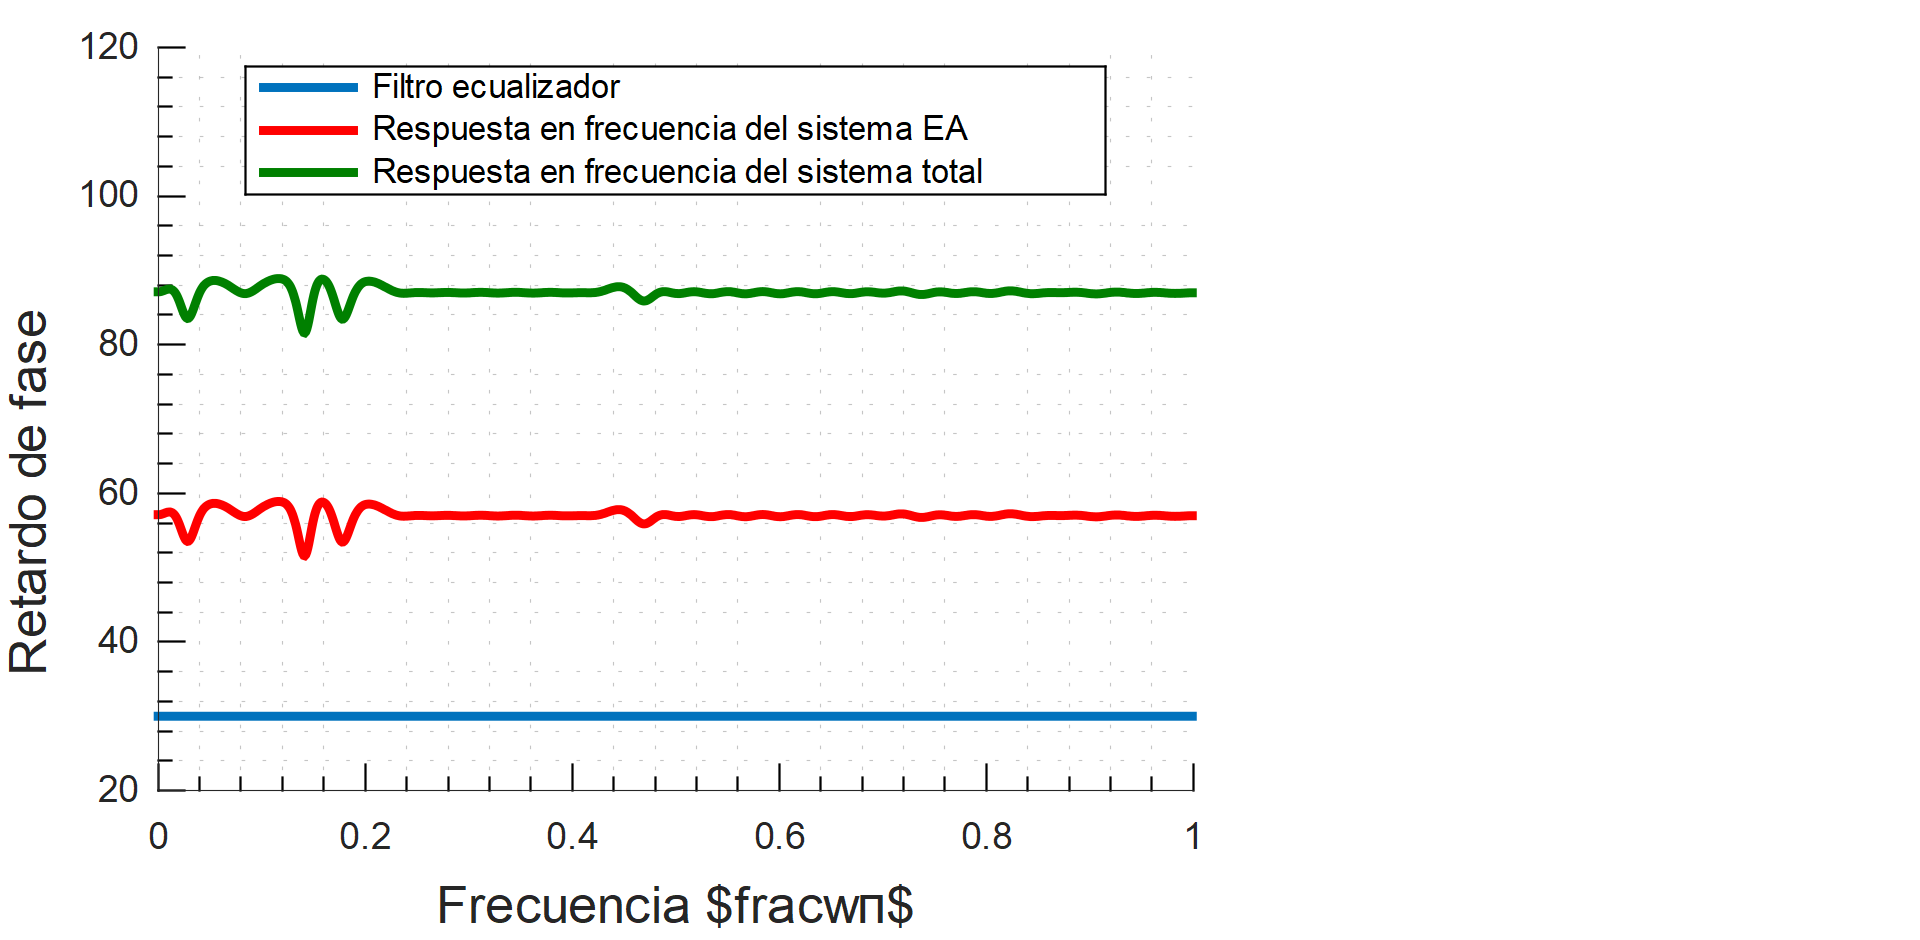
\includegraphics[width=0.9\textwidth]{P12b_retardo_fase.png}
%		\caption{\label{fig:P12b_retardo_fase}Retardo de fase que introduce el filtro ecualizador, el sistema EA y el sistema total.}
%	\end{figure}
	
	Por tratarse del diseño de un filtro de fase lineal, se esperaba aquí también observar un retardo de fase constante. En este método se obtuvo un retardo de 30, un valor menor que con el método de ventanas aplicado (45) a causa de que el orden del filtro es menor. Más allá del valor absoluto del retardo, es de importancia notar que el valor es constante para todas las frecuencias en el rango audible; para aplicaciones de audio, un retardo de fase variable con la frecuencia modifica la forma en que se escucharán las pistas que pasen por el sistema.
	

% Ventajas y desventajas respecto del metodo de 2.1.1

